\documentclass[british]{beamer}

\usepackage{default}
\usepackage[british]{babel}
\usepackage{epstopdf}
\usetheme{Madrid}
\usepackage{graphicx}
\usepackage{dirtytalk}
\usepackage{csquotes}
\usepackage{wrapfig}
\usepackage{tikz}
\usepackage{smartdiagram}
\usepackage{amsmath}
\usepackage{hyperref}


\begin{document}
%
\title[Document Semantic Similarity]
{Document Semantic Similarity}

\subtitle{TIS Project}

\author[A. Pirovano, F. Picciotti]
{Alberto Pirovano \and Francesco Picciotti}

\institute[PoliMi]
{
	Politecnico di Milano
}

\logo{
	
\includegraphics[height=1.7cm,trim={0 2cm 4.5cm 2cm},clip]
	{./Imgs/Politecnico-di-Milano-3-m8qw.eps}
	}

\AtBeginSection[]
{
	\begin{frame}
		\frametitle{Outline}
		\tableofcontents[currentsection, currentsubsection]
	\end{frame}
}

\AtBeginSubsection[]{
	\begin{frame}
		\frametitle{Outline}
		\tableofcontents[currentsection, currentsubsection]
	\end{frame}
}

\maketitle

\section{State of art}

\begin{frame}{Introduzione}
	Le tecniche adottate attualmente per trovare la \textbf{similitudine semantica tra testi} si basano su tre approcci:
	\begin{enumerate}
		\item NLP Tradizionale
		\item Vector Space Model
		\item Deep Learning based 
	\end{enumerate}
\end{frame}
	
\subsection{NLP tradizionale}
	
\begin{frame}{NLP Tradizionale}
	Questo approccio si basa sull'utilizzo delle tradizionali tecniche di \textbf{Natural Language Processing} e si costituisce dei seguenti step:
	\begin{itemize}
		\item Cleaning dei dati
		\item Pos-Tagging
		\item Stemming o Lemmatisation
		\item Parsing
		\item Ontologia
	\end{itemize}
	Tuttavia, dato che il nostro lavoro \`{e} molto \textbf{sensibile} e \textbf{dipendente} dalla qualit\`{a} dei tool utilizzati, abbiamo trovato alcune consistenti \textbf{criticit\`{a}} riguardanti:
	\begin{itemize}
		\item \textbf{L'affidabilit\`{a}} del Pos-Tagger italiano di TreeTagger
		\item \textbf{Reperire} una Ontologia e un parsing tool per la  lingua italiana
	\end{itemize}
\end{frame}

\begin{frame}{NLP Tradizionale}
	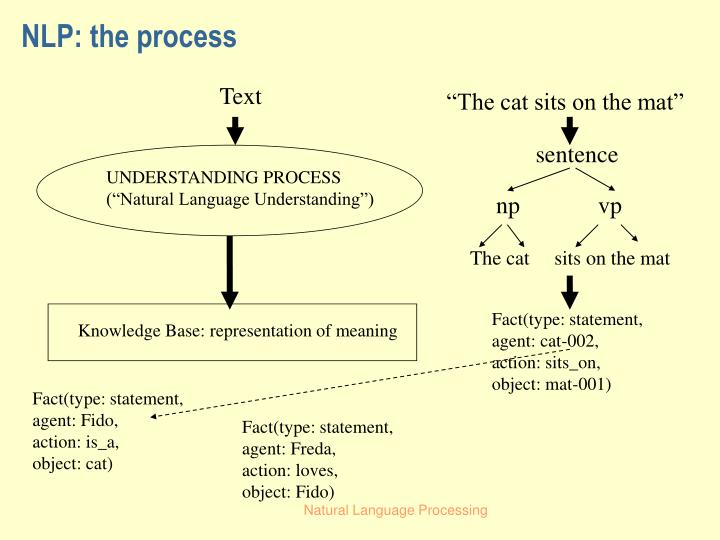
\includegraphics[width=0.9\textwidth, height=0.85\textheight]{./Imgs/nlp-the-process.jpg}
\end{frame}
	
\subsection{Vector Space Model}
	
\begin{frame}{Vector Space Model - Explanation}
	\begin{wrapfigure}{r}{0.4\textwidth}
		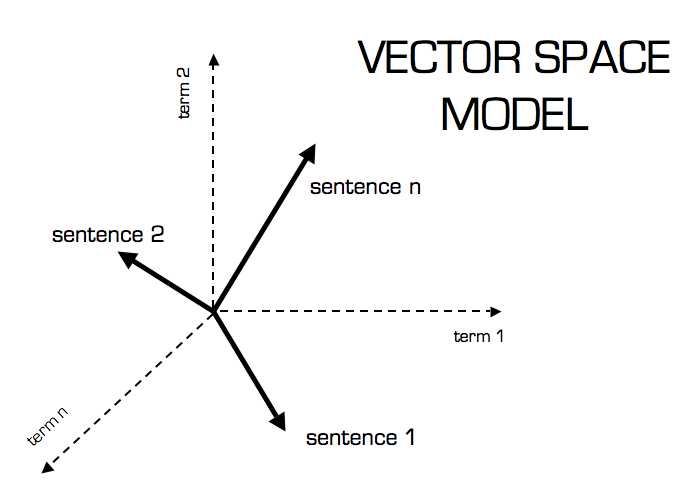
\includegraphics[width=1.1\linewidth,height=0.4\textwidth]{./Imgs/vector_space.png}
	\end{wrapfigure}	
	Differentemente dal precedente, questo approccio ha le sue basi nello sviluppo di una \textbf{rappresentazione geometrica e vettoriale} per i documenti testuali.
	\textbf{Documenti e query} sono rappresentati da vettori con un numero di elementi pari al numero di termini presenti nel vocabolario.
	Tipicamente i termini sono le \textbf{parole distinte} presenti nell'insieme di documenti.
	A valle di questa rappresentazione vengono spesso utilizzate le \textbf{operazioni vettoriali} per confrontare due \textbf{documenti}.
\end{frame}

\begin{frame}{Vector Space Model - Encoding}
	Nel vector space model proposto da \textbf{Salton, Wong and Yang} i vettori sono composti da \textbf{weights}, ognuna associata ad un termine del dizionario e calcolata tramite \textbf{tf-idf}.\par
	Considerando un \textbf{documento \(d_j\)}, questo viene rappresentato tramite un \textbf{vettore \(d_j\)}: \par
	\begin{itemize}
		\item \(d_j = (w_{1,j}, w_{2,j}, ..., w_{t,j})\) \textbf{dove}:
		\(w_{i,j} = tf_{t,d} * \log_{}{\frac{|D|}{|\left \{d' \in D | t \in d'\right \}|}}\)
	\end{itemize}
\end{frame}

\begin{frame}{Vector Space Model - LSA}
	
	\textbf{Latent Semantic Analysis}, anche detta LSI in information retrieval, \`{e} una tecnica di \textbf{Topic Modelling} che si colloca a valle del \textbf{document encoding} con \textbf{tfidf}. 
	
	\`{E} una tecnica di \textbf{feature extraction} che permette di migliorare significativamente la qualit\`{a} di un lavoro di \textbf{clustering}.
	
	Questa procedura viene usata per generare una categorizzazione di un \alert{set di documenti} in un \alert{set di topic} o anche per osservare le parole che descrivono un certo topic.
	
	Si basa sulla creazione di una \textbf{Document-Term Matrix} nella quale le \textbf{righe} rappresentano le parole del \textbf{Bag Of Words} e ha una \textbf{colonna} per \textbf{documento} nel corpora.
	
	Il cuore di questa procedura sta nella \textbf{riduzione della dimensionalit\`{a}} di questa matrice tramite \textbf{SVD}.
	
\end{frame}

\begin{frame}{Vector Space Model - LSA - SVD}
	\begin{itemize}
		\item \textbf{U: }ogni riga rappresenta una parola, mentre ogni colonna rappresenta una \textbf{dimensione nel latent space}; le colonne sono \textbf{ortogonali} l'una all'altra e sono \textbf{ordinate} in base alla varianza dei dati lungo di esse.
	\end{itemize}
	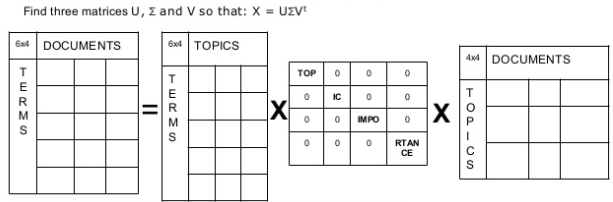
\includegraphics[width=0.9\textwidth,
	 height=0.4\textheight]{./Imgs/LSA1}\\
	 \`{E} importante sottolineare che usando solo \textbf{k} delle \textbf{m} dimensioni\\ latenti si ottiene una \textbf{approssimazione} di \textbf{X}.
\end{frame}

\begin{frame}{Vector Space Model - LSA}
	Questa procedura ci permette di:
	\begin{itemize}
		\item \textbf{Estrarre} quanti topic desideriamo da un set di documenti.
		\item \textbf{Conoscere} la rilevanza di un certo topic dopo averlo estratto, in questo modo siamo in grado di fermare il processo di estrazione quando i topic cominciano a diventare poco significativi.
		\item \textbf{Categorizzare} documenti in topic
		\item \textbf{Descrivere} topics con le parole del \textbf{Bag Of Words}.
	\end{itemize}
\end{frame}

\begin{frame}{Vector Space Model - LSA - Example}
	In questo esempio possiamo osservare la riduzione di dimensionalit\`{a}:
	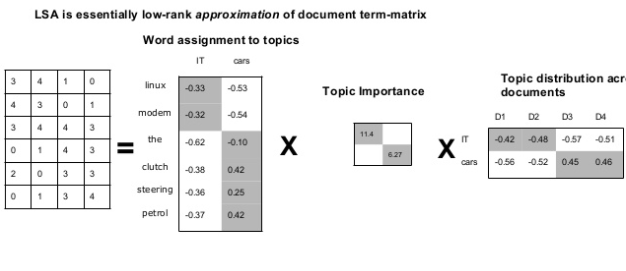
\includegraphics[width=0.9\textwidth, height=0.5
	\textheight]{./Imgs/LSA2}\\
	Il processo di LSA permette di costruire le 3 matrici che vediamo sopra, ognuna con una sua utilit\`{a}:
	\begin{enumerate}
		\item \textbf{Word assignment to topics}
		\item \textbf{Topic importance}
		\item \textbf{Topic distribution across documents}
	\end{enumerate}
\end{frame}

\begin{frame}{Vector Space Model - LSA - Example}
	Ipotizzando un numero di topics pari a 100 e la cardinalit\`{a} del \textbf{Bag of Words} pari a 5000, per ottenere la rappresentazione dei documenti in termini di topics, cio\`{e} un vettore \textbf{z}, dobbiamo:
	\begin{enumerate}
		\item \textbf{Vettorizzare} un documento in \textbf{x}.
		\item \textbf{Proiettare} il \textbf{tfidf} vector \textbf{x} sul topic space.
	\end{enumerate}
	Se definiamo la matrice \(U = (Word assignment to topics)^T\) possiamo visualizzare la \textbf{proiezione} in questo modo:
	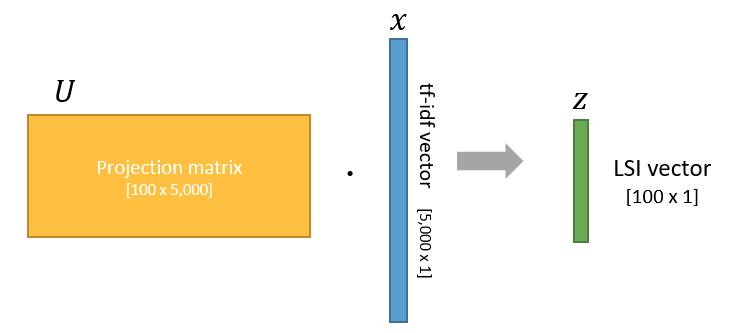
\includegraphics[width=0.9\textwidth, height=0.5\textheight]{./Imgs/LSI}

\end{frame}

\begin{frame}{Vector Space Model - Algorithm}
	Riassumendo, possiamo individuare i seguenti \textbf{passaggi}:
	\begin{enumerate}
		\item Cleaning dei dati (Stemming o Lemmatisation)
		\item Vectorization using TF/IDF (\textbf{x} nella figura nella slide precedente)
		\item LSA (optional) (\textbf{z} nella figura precedente)
		\item Clustering using similarity measure (Cosine, Pearson, ...) tra \textbf{x} vectors o \textbf{z} vectors
	\end{enumerate}
\end{frame}

\begin{frame}{Vector Space Model - LSA - Performance}
	Come possiamo vedere nella figura, utilizzare le classiche tecniche di \textbf{clustering} senza \textbf{LSA} pu\`{o} portare una riduzione rilevante delle \textbf{performances}:
	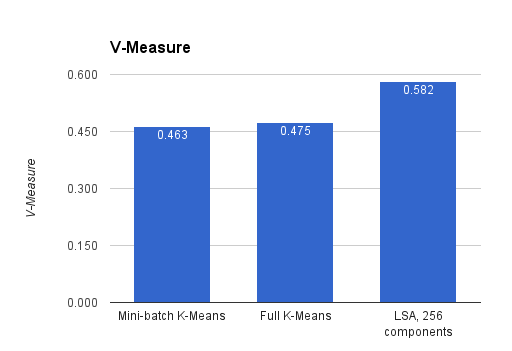
\includegraphics[width=0.9\textwidth, height=0.7\textheight]{./Imgs/LSAperf}
\end{frame}

\begin{frame}{Vector Space Model (con LSA) - Pros and Cons}	
	\begin{columns}
		\column{0.65\textwidth}
		\underline{Cons:}
		\begin{itemize}
			\item Non adatto a trattare \textbf{lunghi documenti}, infatti a causa della alta \textbf{dimensionalit\`{a}} il valore \textbf{tfidf} dei componenti si riduce, riducendo di conseguenza il \textbf{dot-product}.(\alert{LSA fixes})
			\item \textbf{Fortemente sensibile a Falsi Negativi}, infatti documenti nello stesso \textbf{contesto} ma con diversa terminologia non saranno considerati simili.(\alert{LSA fixes})
			\item \alert{Perde \textbf{l'ordine delle parole}}.
			\item \textbf{Pre-processing} dipendente.
			\item \textbf{\alert{Le dimensioni generate possono essere difficili da interpretare}}, sensate matematicamente ma non dal punto di vista del natural language
		\end{itemize}
		\column{0.32\textwidth}
		\\
		\underline{Pros:}
		\begin{itemize}
			\item Modello semplice basato sull'\textbf{algebra}.
			\item Le \textbf{weights} non sono binarie.
			\item Permette di calcolare un grado di \textbf{similarit\`{a} continuo}.
		\end{itemize}
	\end{columns}
\end{frame}

\begin{frame}{Vector Space Model - Limiti}
	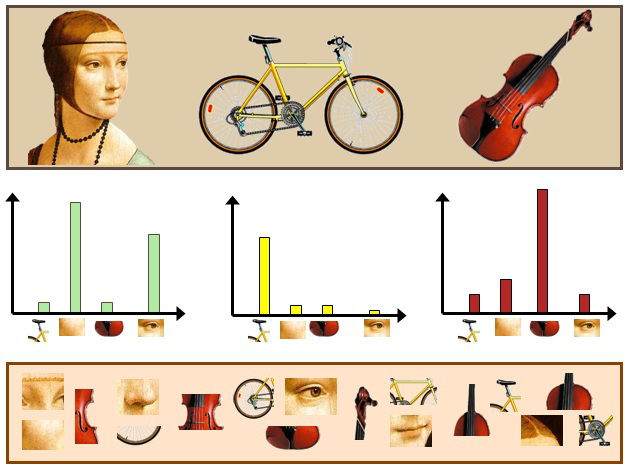
\includegraphics[width=0.9\textwidth, height=0.8\textheight]{./Imgs/bow-example.jpeg}
\end{frame}

\subsection{Deep Learning}

\begin{frame}{Deep learning based}
	
	Il terzo approccio che proponiamo \`{e} molto diverso dai precedenti, infatti si basa sull'utilizzo di \textbf{neural networks}.
	La fondamentale differenza \`{e} che, mentre il secondo \textbf{definiva un algoritmo} per determinare le rappresentazioni vettoriali delle parole (tfidf), questo \textbf{definisce una neural network} con la task di imparare quell'algoritmo dai dati.
	Questa \textbf{NN} pu\`{o} essere \textbf{costruita} in due diversi modi, ognuno dei quali descrive \textbf{come} imparare la \textbf{word-representation} per ogni parola:
	\begin{itemize}
		\item \textbf{Continous Bag Of Words model}
		\item \textbf{Skip Grammar model}
	\end{itemize}
	Dato che il processo di apprendimento \`{e} \textbf{unsupervised}, questi modelli permettono di \textbf{determinare la task} tramite la definizione di un target per ogni input.
\end{frame}
	
\begin{frame}{Deep Learning based}
	Questa tecnica quindi si basa su 3 ambiti:
	\begin{figure}[!hf]
		\centering
		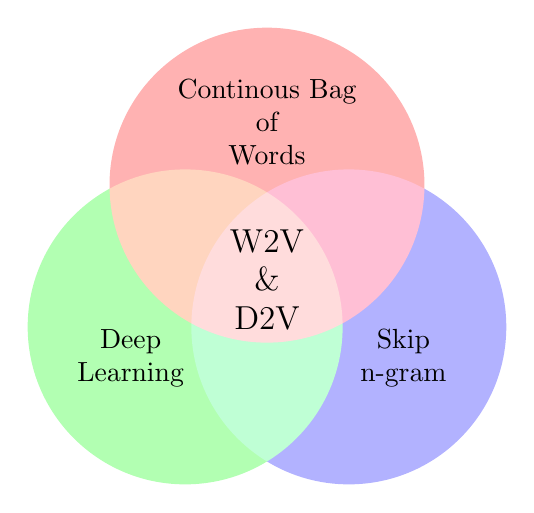
\begin{tikzpicture}
		\begin{scope}[blend group = soft light]
		\fill[red!30!white]   ( 90:1.2) circle (2);
		\fill[green!30!white] (210:1.2) circle (2);
		\fill[blue!30!white]  (330:1.2) circle (2);
		\end{scope}
		\node at ( 90:2)    
		[font= \normalsize, align= center]
		{Continous Bag \\ of \\ Words};
		\node at ( 210:2)   
		[font= \normalsize, align= center]
		{Deep \\ Learning};
		\node at ( 330:2)   
		[font= \normalsize, align= center]
		{Skip \\ n-gram};
		\node [font=\large, , align= center] {W2V \\\& \\D2V};
		\end{tikzpicture}
	\end{figure}
\end{frame}
	
\begin{frame}{Deep Learning based: Word2Vec \& Doc2Vec}
	Questo metodo \`{e} stato implementato da \textbf{Google} sotto il nome di \textbf{Word2Vec} e \textbf{Doc2Vec}.
	Il primo permette di determinare le \textbf{relazioni semantiche} che un particolare \textbf{corpus di testi} assegna ad un \textbf{Bag Of Words} di parole.
	\textbf{Doc2Vec} invece \`{e} una tecnica che si configura come una \textbf{estensione di Word2Vec} la quale, preso in ingresso un set di documenti (corpora), genera un \textbf{grado di similarit\`{a}}.
\end{frame}

\begin{frame}{Deep Learning based - Pros and Cons}
	Dopo una ampia \textbf{discussione}, seguita da una approfondita \textbf{analisi critica} di questi due approcci, siamo giunti alle seguenti \textbf{conclusioni}, che in termini di pro e contro si possono riassumere nel seguente modo:
	\begin{columns}
		\column{0.5\textwidth}
		\\
		\underline{Pros:}
		\begin{itemize}
			\item Molto meno dipente da un preprocessing
			\item Combina il metodo \textit{Geometrico} con quello \textit{NLP Tradizionale}
			\item \textbf{Non sfrutta una ontologia, ma la \alert{crea}} 
			\item \textbf{\alert{Language independent}}
			\item \textbf{\alert{Tiene in considerazione anche l'ordine delle parole}}, \textbf{Context-aware}
		\end{itemize}
		\column{0.5\textwidth}
		\underline{Cons:}
		\begin{itemize}
			\item Tecnica \textbf{unsupervised}
			\item Necessit\`{a} di un esperto per \textbf{validare} la similarit\`{a}
			\item Pu\`{o} risultare in \textbf{GIGO} system (Garbage In Garbage Out)
		\end{itemize}
	\end{columns}
\end{frame}
	
\section{Data Preparation}

\begin{frame}{Dataset}
	\begin{displayquote}
		"Preprocessing is 80\% of NLP work"
		 
		\begin{flushright}
			\textit{Lev Konstantinovskiy}
		\end{flushright}
	\end{displayquote}
	Il \textbf{dataset} si suddivide in due corpora: 
	\begin{itemize}
		\item il corpus del \textbf{Sole 24 Ore} con 3265 articoli, di cui 31 non hanno body
		\item il corpus di \textbf{Radiocor} con 6916 articoli
	\end{itemize}
	Il corpus prima del \textbf{preprocessing} contiene quindi 10150 articoli. \par
	Togliendo i \textbf{duplicati} otteniamo 9283 articoli, cio\'{e} ci sono 867 articoli duplicati.
\end{frame}

\subsection{Preprocessing}

\begin{frame}{Pipeline completa}
	\begin{center}
		\smartdiagramset{
			module minimum width= 5cm, 
			text width= 4.5cm,
			font= \tiny,
			set color list={blue!50!cyan,green!60!lime,orange!50!red,red!80!black},
			back arrow disabled=true}
		\smartdiagram[flow diagram: horizontal]{Cleaning del testo,Tokenizzazione e rimozione punteggiatura, Rimozione stopwords e POS-tagging del testo,Lemmatizzatione,Merge di verbi passivi composti}
	\end{center}
\end{frame}

\subsection{Cleaning del testo}

\begin{frame}{Cleaning pipeline}
	\begin{center}
			\smartdiagramset{
				module minimum width= 5cm,
				module minimum height= 0.1cm, 
				text width= 5cm,
				module y sep= 0.8cm,
				font= \tiny,
				set color list={blue!50!cyan,green!60!lime,orange!50!red,red!80!black},
				back arrow disabled=true}		
			\smartdiagram[flow diagram: vertical]{Lowercase di ogni lettera, Escape di caratteri unicode non stampabili, Tokenizzazione numeri percentuali, Rimozione preposizioni contratte, Tokenizzazione parola s24, Unificazione di espressioni di quantit\`{a}, Rimozione di intestazione di articolo, Rimozione di interruzione pagina, Rimozione chiusura aricolo, Rimozione urls e tags html}
	\end{center}
\end{frame}

\section{Word2Vec}

\begin{frame}{Word2Vec - Task}
	\textbf{Word2Vec} \`{e} un gruppo di modelli che vengono usati per generare \textbf{word-embeddings} da \textbf{unstructured text}. Per questo scopo viene usata una \textbf{\alert{two-layers neural network}} che viene trainata per ricostruire il \textbf{contesto linguistico} delle parole.
	\begin{itemize}
		\item \textbf{Input: }\textbf{corpus} di testo
		\item \textbf{Output: }\textbf{vector-space}
	\end{itemize}
	Ogni parola \textbf{unica nel corpus} verr\`{a} rappresentata con un vettore nel \textbf{vector-space}.
	L'algoritmo generer\`{a} degli word-embeddings tali per cui parole che condividono lo stesso contesto nel corpus risulteranno vicine nel \textbf{vector space}.
\end{frame}

\begin{frame}{Word2Vec - Idea}
	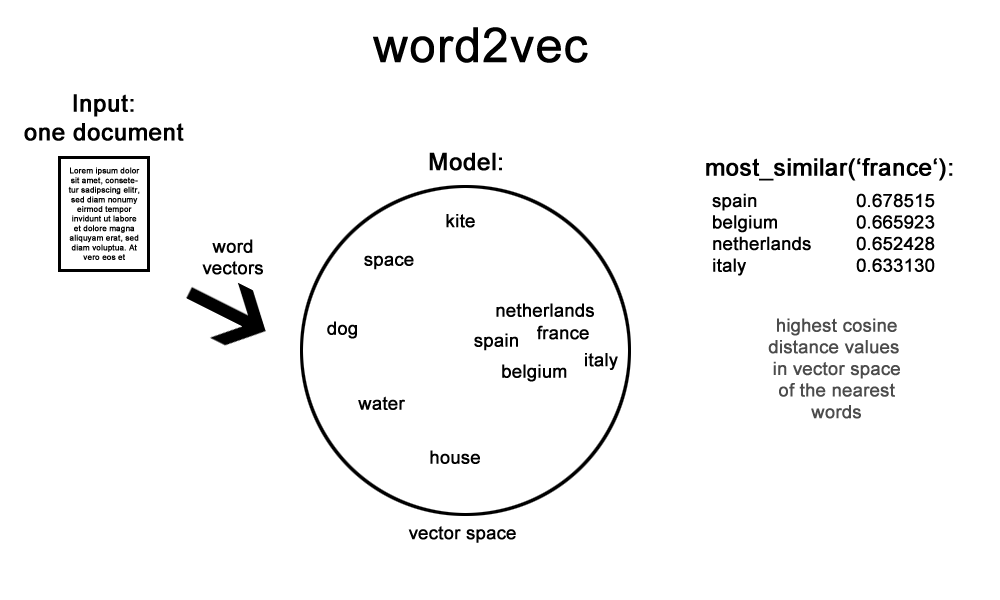
\includegraphics[width=0.8\linewidth]{./Imgs/word2vec-working.png}
\end{frame}

\begin{frame}{Word2Vec - From unsupervised to supervised}
	Questa task pu\`{o} essere definita in due modi:
	\begin{enumerate}
		\item \textbf{Skip Grammar} - predire il \textbf{contesto} data la parola in input
		\begin{itemize}
			\item \textbf{Input: }focus-word
			\item \textbf{Target: }context-words
		\end{itemize}
		\item \textbf{Continous Bag Of Words} - predire la parola in input dato il \textbf{contesto}
		\begin{itemize}
			\item \textbf{Input: }context-words
			\item \textbf{Target: }focus-word
		\end{itemize}
	\end{enumerate}
	Definendo input e target pairs abbiamo definito un \textbf{supervised problem}, che affronteremo usando \textbf{logistic classifiers} ( logistic regression ).
\end{frame}

\begin{frame}{Word2Vec - Encoding}
	Gli \textbf{input-target pairs} sono rappresentati tramite \textbf{One Hot Encoding}, mentre l'\textbf{output} della NN sar\`{a} un vettore di probabilit\`{a} di dimensione pari al numero di parole del \textbf{vocabolario}.\\
	Di conseguenza se abbiamo un vocabolario di \textbf{dimensionalit\`{a} V} avremo dei \textbf{vectors} costituiti da V elementi di cui un 1 e gli altri 0.
\end{frame}

\begin{frame}{Word2Vec - Context}
	In entrambi i casi \`{e} necessario definire un \textbf{context} per la parola in input, che identifichiamo con un parametro chiamato \textit{c = windowsize}.
	Tramite questa \textit{windowsize}, una volta fissata una \textbf{input word/focus word}, chiamiamo \textbf{\alert{context}} l'insieme delle \textit{c} parole prima della input word pi\`{u} le \textit{c} parole dopo la input word.
	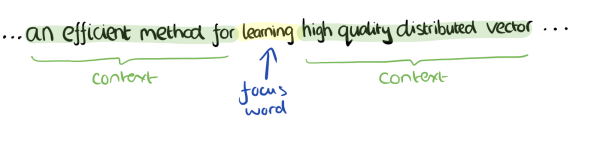
\includegraphics[width=1\linewidth,height=0.2\textwidth]{./Imgs/context}\\
	Terminologia:
	\begin{itemize}
		\item V = numero di elementi nel vocabolario
		\item N = numero di weights per word embeddings
		\item c = window size
	\end{itemize}
\end{frame}

\begin{frame}{Word2Vec - Skip Grammar}
	\begin{columns}
		\begin{column}{0.4\textwidth}
			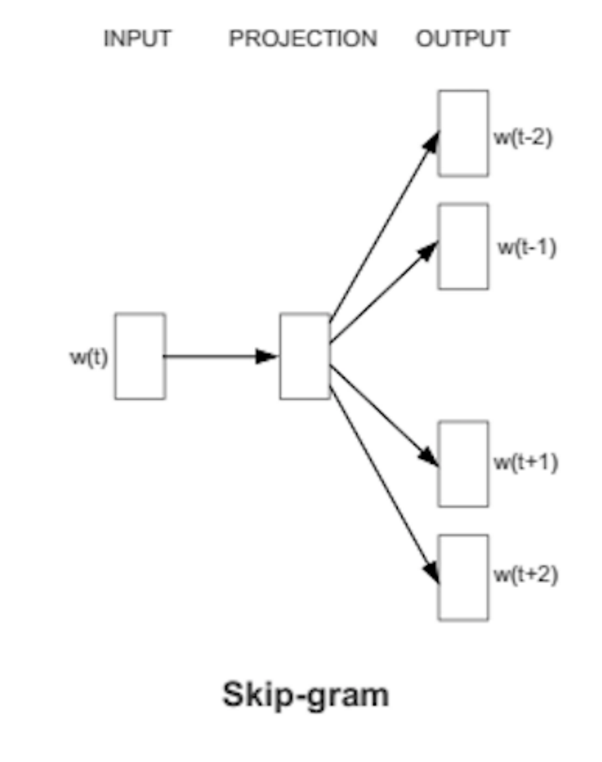
\includegraphics[width=1.1\linewidth,height=1.4\textwidth]{./Imgs/skip.png}
		\end{column}
		\begin{column}{0.6\textwidth}
			Data una sequenza di \textbf{training words} \(w_1, w_2, ... w_M\), con \(M = trainingsetsize\), il \textbf{training objective} di questo modello \`{e} trovare il parametro \(\theta\) che massimizza la \textbf{Log-Likelihood}:
			\\~\\
			\(L =	\frac{1}{M}\cdot\sum_{m=1}^{M}\sum_{-c<j<c,j\neq0}\log p(w_{m+j}|w_{m})\)
			\\~\\
			Ogni classification task, data una \textbf{focus word} \(w_m\) e una parola del contesto \(w_{m+j}\), calcola \textbf{la probabilit\`{a}} \(p(w_{m+j}|w_{m})\).
			\begin{itemize}
				\item Di conseguenza per ogni input \\vector definiamo circa \textbf{2c logistic\\ classifiers}.
			\end{itemize}
		\end{column}
	\end{columns}
\end{frame}

\begin{frame}{Word2Vec - CBOW}
	\begin{columns}
		\begin{column}{0.4\textwidth}
			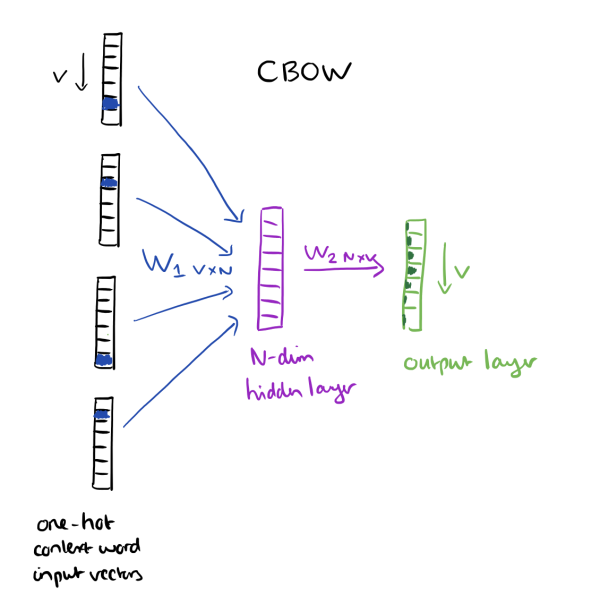
\includegraphics[width=1.1\linewidth,height=1.4\textwidth]{./Imgs/cbow}
		\end{column}
		\begin{column}{0.6\textwidth}
			Data una sequenza di \textbf{training words} \(w_1, w_2, ... w_M\), con \(M = trainingsetsize\), il \textbf{training objective} di questo modello \`{e} trovare il parametro \(\theta\) che massimizza la \textbf{Log-Likelihood}:
			\\~\\
			\(L = \frac{1}{M}\cdot\sum_{m=1}^{M}\log p(w_{m}|w_{m-c}, ... , w_{m+c})\)
			\\~\\
			Ogni classification task, date una serie di \textbf{context words}, le  calcola \textbf{la probabilit\`{a}} \(p(w_{m}|w_{m-c}, ... , w_{m+c})\).
			\begin{itemize}
				\item Di conseguenza per ogni input\\ vector definiamo \textbf{1 logistic\\ classifier}.
			\end{itemize}
		\end{column}
	\end{columns}
\end{frame}

\begin{frame}{Word2Vec - Matrices}
	Le due \textbf{weight matrices} \(W_1 [V\cdot N]\) e \(W_2 [N\cdot V]\) sono della stessa dimensione e contengono entrambe un \textbf{word-embedding vector} per ogni vocabulary word.\\
	La \textbf{prima} fornisce la \textbf{\alert{input vector representation}} delle vocabulary words e la \textbf{seconda} fornisce la \textbf{\alert{output vector representation}} delle vocabulary words.\\
	In generale data una parola \(w \in V\):
	\begin{itemize}
		\item \(v_w\) \`{e} la sua \textbf{input representation}, vale a dire un vettore \([1 \cdot N]\) relativo a \(w\) che otteniamo da \(W_1\):
		\item \(v_w'\) \`{e} la sua \textbf{output representation}, vale a dire un vettore \([1 \cdot N]\) relativo a \(w\) che otteniamo da \(W_2\):
	\end{itemize}
\end{frame}

\begin{frame}{Word2Vec - Hidden layer}
	\`{E} interessante notare come, dato un input \textbf{OHE}, l'\textbf{hidden layer} funga da \textbf{lookup table} per selezionare il \textbf{word vector} relativo alla input word, \(v_{wInput}\)(no activation function).
	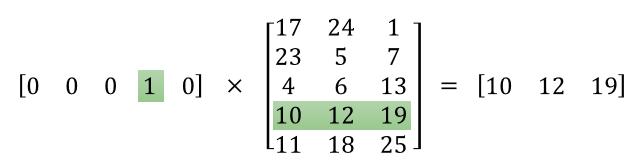
\includegraphics[width=1\linewidth,height=0.25\textwidth]{./Imgs/lookup_table}\\
	Possiamo quindi dire che:
	\begin{itemize}
		\item \textbf{Skip Grammar: }L'\textbf{output dell'hidden layer} (\(v_{wInput}\)) \`{e} il \textbf{word vector} relativo all'\textbf{input word}, in questo caso \(v_{wInput} = [10, 12, 19]\).
		\item \textbf{CBOW: }Ogni \textbf{OHE} vector delle parole del contesto effettua il lookup e ottiene il word-embedding dalla matrice \(W_1\). Successivamente\\ viene fatta una media degli word embeddings ottenuti in modo\\ tale da ottenere l'output dell'hidden layer (\(v_{wAverage}\)).
	\end{itemize}
\end{frame}

\begin{frame}{Word2Vec - Probabilistic view}
	Considerando i due tipi di approccio, possiamo quindi esplicitare le \textbf{probabilit\`{a} scalari} utilizzate nella funzione di costo, con \(w_{m} = w_{Input}\):
	\\~\\
	\begin{itemize}
		\item \textbf{Skip Grammar: }
		\(p(w_{m+j}|w_{m}) = \frac{exp(v_{w_{m+j}}'^T \cdot v_{w_{Input}}^T)}{\sum_{i=1}^{V}exp(v_{w_i}'^T \cdot v_{w_{Input}}^T)}\)
		\item \textbf{CBOW: }
		\(p(w_{m}|w_{m-c}, ... , w_{m+c}) = \frac{exp(v_{w_{m}}'^T \cdot v_{wAverage}^T)}{\sum_{i=1}^{V}exp(v_{w_i}'^T \cdot v_{wAverage}^T)}\)
	\end{itemize}
	Tecnicamente il \textbf{vettore di probabilit\`{a}} che viene generato dalla rete, dato un \textbf{input vector} o un \textbf{input average}, \`{e}:
	\\~\\
	\begin{itemize}
		\item \textbf{Skip Grammar: }
		\(y_{t+j} = \frac{exp(W_2^T \cdot v_{wInput}^T)}{\sum_{i=1}^{V}exp(v_{w_i}'^T \cdot v_{wInput}^T)}\)
		\item \textbf{CBOW: }
		\(y_t = \frac{exp(W_2^T \cdot v_{wAverage}^T)}{\sum_{i=1}^{V}exp(v_{w_i}'^T \cdot v_{wAverage}^T)}\)
	\end{itemize}
\end{frame}

\begin{frame}{Word2Vec - Output layer}
	L'\textbf{output layer} si compone di due operazioni:
	\begin{enumerate}
		\item Calcolare lo score dell'input vector, \(scoreVec = v_{wInput}^T \cdot W_2\) per \textbf{Skip Grammar} o \(scoreVec = v_{wAverage}^T \cdot W_2\) per \textbf{CBOW}.
		\item \textbf{Multi-class classification} attraverso \textbf{softmax}, \(softmax(scoreVec) = \frac{e^{scoreVec}}{\sum_{i=1}^{V}e^{scoreVec_i}}\)
	\end{enumerate}
	Dove \(V = sizevocabulary\), \(scoreVec_i\) \`{e} l'i-esimo componente di \(scoreVec\) e \(e^{vector}\) rappresenta l'esponenziale element by element.
	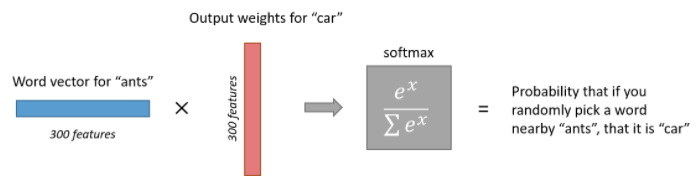
\includegraphics[width=0.9\linewidth,height=0.25\textwidth]{./Imgs/output_layer}
\end{frame}

\begin{frame}{Word2Vec - Parameters Learning - Loss}
	Il \textbf{loss} viene definito come \textbf{una media} dei \textbf{loss relativi} ad ogni \textbf{training sample}, nel nostro caso un training sample \`{e} una \textbf{parola nel corpus}.\\
	\begin{columns}
		\begin{column}{0.3\textwidth}
			
		\end{column}
		\begin{column}{0.4\textwidth}
			\\~\\
			\(L = \frac{1}{M} \cdot \sum_{m=1}^{M} L_m\)
			\\~\\
		\end{column}
		\begin{column}{0.3\textwidth}
			
		\end{column}
	\end{columns}
	L'espressione del loss in questi termini serve solo a \textbf{visualizzare} il suo valore durante le \textbf{iterazioni dell'algoritmo}.\\
	Un \textbf{epoch} (iterazione) della procedura di training consiste nell'effettuare per ogni \textbf{training sample} la procedura di \textbf{forward e back propagation}.\\
	Per ogni sample in un \textbf{epoch} vengono quindi aggiornate tutte le \textbf{weights} del modello.\\
	Ad ogni \textbf{epoch} la massimizzazione del \textbf{loss} sar\`{a} effettuata considerando il loss \(L_m\) relativo a sample che sta attraversando il network. 
	
\end{frame}

\begin{frame}{Word2Vec - Parameters Learning}
	Cominciamo considerando il caso di \textbf{CBOW} in cui abbiamo una sola parola nel contesto, vale a dire il modello dovr\`{a} predire la \textbf{focus word} data \textbf{\alert{una}} parola nel \textbf{contesto}.
	\\~\\
	\begin{columns}
		\begin{column}{0.15\textwidth}
		
		\end{column}
		\begin{column}{0.7\textwidth}
			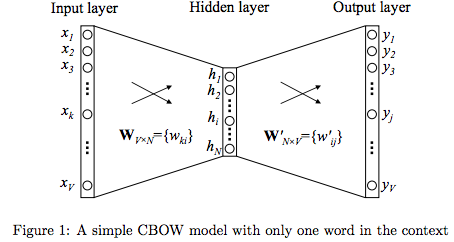
\includegraphics[width=1\linewidth,height=0.55\textwidth]{./Imgs/cbow_onecontext}
		\end{column}
		\begin{column}{0.15\textwidth}
		
		\end{column}
	\end{columns}
	In questa figura \(W = W_1\) e \(W' = W_2\).
\end{frame}

\begin{frame}{Word2Vec - Parameters Learning - CBOW - \(L_m\)}
	Considerando il \textbf{training sample m} che attraversa il network e ipotizzando \(w_{m-1}\) l'unica parola nel contesto di \(w_{m}\);
	\begin{gather*}
		\begin{split}
		L_m &= \log p(w_{m}|w_{context}) = 
		\log \left( \frac{exp(v_{w_{m}}'^T \cdot v_{w_{context}}^T)}{\sum_{i=1}^{V} exp(v_{w_{i}}'^T \cdot v_{w_{context}}^T)} \right) = 
		\\
		&= \log \left( \frac{exp(v_{w_{m}}'^T \cdot h)}{\sum_{i=1}^{V} exp(v_{w_{i}}'^T \cdot h)} \right) =
		\log \left( \frac{exp(u_m)}{\sum_{i=1}^{V} exp(u_i)} \right) =
		\\
		&= \log \left( exp(u_m) \right) - \log \left( \sum_{i=1}^{V} exp(u_i) \right) =
		\\
		&= u_m - \log \left( \sum_{i=1}^{V} exp(u_i) \right) = -E
		\end{split}
	\end{gather*}
	Quindi l'errore commesso per \textbf{UN SOLO TRAINING SAMPLE} \`{e}:
	\begin{columns}
		\begin{column}{0.3\textwidth}
			
		\end{column}
		\begin{column}{0.4\textwidth}
			\(E = -\log p(w_{m}|w_{m-1})\)
		\end{column}
		\begin{column}{0.3\textwidth}
			
		\end{column}
	\end{columns}
\end{frame}

\begin{frame}{Word2Vec - Parameters Learning - Forward Propagation}
	Chiamiamo:
	\begin{itemize}
		\item \(u_i\) con \(i \in {1,2,..,V}\) lo score calcolato per la parola \(i\).
		\item \(h_i\) con \(i \in {1,2,..,N}\) l'output del i-th neurone dell'hidden layer.
		\item \(y_i\) con \(i \in {1,2,..,V}\) l'output del i-th neurone dell'output layer.
		\\~\\
	\end{itemize} 
	Considerando un \textbf{OHE} vector in input \(x_{context}\) di dimensioni \([V,1]\) con il k-th elemento \(x_k \neq 0\), definiamo:
	\begin{itemize}
		\item \(h = \sigma(W^T \cdot x_{context}) = W^T \cdot x_{context} = v_{w_{context}}^T\), vale a dire che la funzione di attivazione per il primo layer \`{e} la funzione identit\`{a} (\textbf{lookup table}).
		\item \(h_i = \sum_{k=1}^{V} x_k \cdot w_{ki}\)
		\item \(u_j = v_{w_j}'^T \cdot h\)
		\item \( y_{j} = p(w_{j}|w_{context}) =  \frac{exp(u_{j})}{\sum_{i=1}^{V} exp(u_i)}\), la probabilit\`{a} a posteriori che\\ \(w_{j}\) \(\in V\) sia la parola campionata nel contesto di \(w_{context}\).
	\end{itemize}
\end{frame}

\begin{frame}{Word2Vec - Parameters Learning - W' (\(W_2\))}
	\begin{gather*}
		\begin{align*}
		\frac{\partial E}{\partial u_j} 
		&= \frac{\partial \left( \log \left( \sum_{i=1}^{V} exp(u_i) \right) - u_m\right)}{\partial u_j} =
		\\
		&= \frac{\partial \left(\log \left( \sum_{i=1}^{V} exp(u_i) \right)\right)}{\partial u_j} - \frac{\partial \left( u_m\right)}{\partial u_j}= 
		\\
		&= \frac{exp(u_j)}{\sum_{i=1}^{V} exp(u_i)} - t_j= &
		\\
		&= y_j -t_j = e_j & \text{dove } 
		t_{j}=\begin{cases}
				1 \quad \text{if } j=m\\
				0 \quad \text{if } j\neq m
			\end{cases}
		\\
		\frac{\partial u_j}{\partial w_{ij}'} &= \frac{\partial \left( v_{w_j}'^T \cdot h\right)}{\partial w_{ij}'} = h_i
		\\
		\frac{\partial E}{\partial w_{ij}'} &= \frac{\partial E}{\partial u_j} \cdot \frac{\partial u_j}{\partial w_{ij}'} = e_j \cdot h_i
		\end{align*}		
	\end{gather*}
\end{frame}

\begin{frame}{Word2Vec - Parameters Learning - W' (\(W_2\))}
	L'aggiornamento dei parametri quindi risulta:
	\begin{gather*}
		\begin{align*}
		w_{ij}'^{(t+1)} &= w_{ij}'^{(t)} - \eta\cdot h_i \cdot e_j &\mathit{i} \in {1,2,..,N} \wedge \mathit{j} \in {1,2,..,V}
		\\
		v_{w_{j}}'^{(t+1)} &= v_{w_{j}}'^{(t)} - \eta\cdot h \cdot e_j &\mathit{j} \in {1,2,..,V}
		\end{align*} 
	\end{gather*}
	\textbf{Di conseguenza ad ogni ciclo vengono aggiornati tutti i pesi della matrice \(W_1\).}
\end{frame}

\begin{frame}{Word2Vec - Parameters Learning - W (\(W_1\))}
	\begin{gather*}
		\begin{split}
		\frac{\partial E}{\partial h_i} &= \sum_{j=1}^{V} \left(\frac{\partial E}{\partial u_j} \cdot \frac{\partial u_j}{\partial h_i}\right) = 
		\sum_{j=1}^{V} \left(e_j \cdot \frac{\partial u_j}{\partial h_i}\right) = 		\\
		&= \sum_{j=1}^{V} \left(e_j \cdot w_{ij}'\right) =
		e \cdot (W_{2_{i}})^T
		\\
		\intertext{Dove \(W_{2_{i}}\) \`{e} la i-esima riga di \(W_2\) (\([1,V]\)), che trasposta da un vettore \([V,1]\), il quale, moltiplicato per un vettore \([1,V]\) da uno scalare.}
		\frac{\partial h_i}{\partial w_{ki}} &= x_k
		\\
		\frac{\partial L_m}{\partial w_{ki}} &= \frac{\partial L_m}{\partial h_i} \cdot \frac{\partial h_i}{\partial w_{ki}} = x_k \cdot e \cdot (W_{2_{i}})^T
		\end{split}
	\end{gather*}
\end{frame}

\begin{frame}{Word2Vec - Parameters Learning - W (\(W_1\))}
	L'aggiornamento dei parametri quindi risulta:
	\begin{itemize}
		\item \( w_{ki}^{(t+1)} = w_{ki}^{(t)} - \eta\cdot x_k \cdot e \cdot (W_{2_{i}})^T\), con \(k \in {1,2,..,V}\) e \(i \in {1,2,..,N}\)
		\item \( W_{1}^{(t+1)} = W_{1}^{(t)} - \eta\cdot x \cdot \left( e \cdot W_{2}^T \right) \)
	\end{itemize}
	Dove \(x \cdot \left( e \cdot W_2^T\right)\) \`{e} di dimensionalit\`{a} \([V,N]\).\\
	Considerando poi che \(x\) \`{e} un \textbf{OHE vector}, solo un coefficiente di \(x\) sar\`{a} \(\neq 0\).
	Di conseguenza questa operazione di aggiornamento lascia inalterate tutte le \textbf{input representation} della matrice \textbf{\(W_1\)} tranne quella corrispondente all'indice \(x_k \neq0\) di \(x\). \\
	Quindi l'unico aggiornamento che avviene \`{e}:
	\begin{itemize}
		\item \( v_{w_{context}}^{(t+1)} = v_{w_{context}}^{(t)} - \eta\cdot \left(e \cdot W_{2}^T\right)\)
	\end{itemize}
	Di conseguenza vediamo una delle particolarit\`{a} di \textbf{word2vec}, vale a dire che \textbf{per ogni parola in input l'aggiornamento di \(W_1\) si limita \\solo al word vector relativo alla input word, in questo caso di\\ \(v_{w_{context}}\)}. 
\end{frame}

\begin{frame}{Word2Vec - Parameters Learning - Batch GD}
	Invece di considerare un solo sample per volta possiamo anche considerare un \textbf{batch} \(X\) di \(M\) samples:
	\begin{itemize}
		\item \(X\) = una \textbf{OHE} riga per ogni \textbf{input sample} in \(M\), \([M,V]\)
		\item \(T\) = una \textbf{OHE} riga per ogni \textbf{target sample} in \(M\), \([M,V]\)
	\end{itemize}
	La \textbf{forward pass} sar\`{a}:
	\begin{itemize}
		\item \(H = X \cdot W_1\)  \([M,N]\)
		\item \(U = H \cdot W_2\),  \([M,V]\)
		\item \(Y = softmax(U)\),  \([M,V]\), row-wise
	\end{itemize}
	La \textbf{back pass} sar\`{a}:
	\begin{itemize}
		\item \( \frac{\partial E}{\partial U} = \frac{1}{M} \cdot \left( Y - T \right) \), \([M,V]\)
		\item \( \frac{\partial E}{\partial W_2} = H^T \cdot\frac{\partial E}{\partial U} \), \([N,V]\)
		\item \(\frac{\partial E}{\partial H} = \frac{\partial E}{\partial U} \cdot W_2^T \), \([M,N]\)
		\item \(\frac{\partial E}{\partial W_1} = X^T \cdot \frac{\partial E}{\partial H}\), \([V,N]\)
	\end{itemize}
\end{frame}

\begin{frame}{Word2Vec - Parameters Learning - Complete CBOW}
	Considerando il modello \textbf{CBOW} con multiple parole nel contesto della parola \(w_{m}\) avremo pochi cambiamenti rispetto al modello appena spiegato.
	\begin{itemize}
		\item \( h = \frac{1}{C} \cdot W_1^T \cdot \left(x_{m-C} + ... + x_{m-2} + x_{m-1} + x_{m+1} + x_{m+2} + ... + x_{m+C} \right)\)
	\end{itemize}
	Di conseguenza il vettore h diventa una media delle input representations delle parole nel contesto.\\
	La procedura si svolge nello stesso modo, tranne per quanto riguarda l'aggiornamento dei pesi della matrice \(W_1\), infatti vengono aggiornate un numero di \textbf{input representation} pari al numero della parole nel contesto:
	\begin{itemize}
		\item \( v_{w_{m-c}}^{(t+1)} = v_{w_{m-c}}^{(t)} - \eta\cdot \frac{1}{C} \cdot \left(e \cdot W_{2}^T\right)\), con \(c \in {C,...,-C} \) e \(c \neq 0\)
	\end{itemize}	
	Per quanto riguarda \(W_2\) invece non cambia niente:
	\begin{itemize}
		\item \( v_{w_{j}}'^{(t+1)} = v_{w_{j}}'^{(t)} - \eta\cdot h \cdot e_j\), con \(j \in {1,2,..,V}\)
	\end{itemize}
\end{frame}

\begin{frame}{Word2Vec - Parameters Learning - Skip Gram - \(L_m\)}
	Considerando il \textbf{training sample m} che attraversa il network e ipotizzando \(w_{m-1}\) l'unica parola nel contesto di \(w_{m}\)
	\begin{gather*}
		\begin{split}
		L_m &= \sum_{-c<j<c,j\neq0}\log p(w_{m+j}|w_{m}) =
		\sum_{-c<j<c,j\neq0} \log \frac{exp(v_{w_{m+j}}'^T \cdot v_{w{m}}^T)}{\sum_{i=1}^{V} exp(v_{w_{i}}'^T \cdot v_{w_{m}}^T)} 
		\\
		&= \sum_{-c<j<c,j\neq0} \log \frac{exp(u_{m+j})}{\sum_{i=1}^{V} exp(u_i)} = 
		\\
		&= \sum_{-c<j<c,j\neq0} \log exp(u_{m+j}) - \sum_{-c<j<c,j\neq0} \log \sum_{i=1}^{V} exp(u_i) =
		\\
		&= \sum_{-c<j<c,j\neq0} u_{m+j} - C \cdot \log \sum_{i=1}^{V} exp(u_i) = -E
		\end{split}
	\end{gather*}
	Quindi l'errore commesso per \textbf{UN SOLO TRAINING SAMPLE} \`{e}:
	\begin{columns}
		\begin{column}{0.2\textwidth}
			
		\end{column}
		\begin{column}{0.6\textwidth}
			\(E = - \sum_{-c<j<c,j\neq0}\log p(w_{m+j}|w_{m})\)
		\end{column}
		\begin{column}{0.2\textwidth}
			
		\end{column}
	\end{columns}
\end{frame}

\begin{frame}{Word2Vec - Parameters Learning - Skip Gram - Forward Propagation}
	Chiamiamo:
	\begin{itemize}
		\item \(u_{c,j'} = u_{j'} = v_{w_{j'}}'^T \cdot h \), per ogni parola nel contesto di \(v_{w_{m}}\), infatti gli output panels condividono la stessa matrice di weights \(W_2\).
		\item \(h = v_{w_{m}}^T\)
	\end{itemize} 
\end{frame}

%TO DO Finire questa formula
%\begin{frame}{Word2Vec - Parameters Learning -Skip Gram - W' (\(W_2\))}
%	\begin{gather*}
%		\begin{split}
%		\frac{\partial E}{\partial u_{m+c,j'}} &= \frac{\partial \left( C \cdot \log \sum_{i=1}^{V} exp(u_i) - \sum_{-c<j<c,j\neq0} u_{m+j}\right)}{\partial u_{m+c, j'}} =
%		\\
%		&= \frac{\partial \left(C \cdot \log \left( \sum_{i=1}^{V} exp(u_i) \right)\right)}{\partial u_{m+c,j'}} - \frac{\partial \left( \sum_{-c<j<c,j\neq0} u_{m+j}\right)}{\partial u_{m+c,j'}}=
%		\\
%		&= \frac{\partial \left(C \cdot \log \left( \sum_{i=1}^{V} exp(u_i) \right)\right)}{\partial u_{m+c,j'}} - t_{m+c,j'}=
%		\end{split}
%	\end{gather*}
%\end{frame}

\begin{frame}{Word2Vec - Fake task}
	L'aspetto interessante di questa tecnica \`{e} che, dopo il training, \textbf{la rete non verr\`{a} utilizzata per la task su cui \`{e} stata addestrata}. Il training serve solo per aggiornare e migliorare i pesi delle matrici \(W_1\) e \(W_2\).
	\begin{itemize}
		\item Quello che ci interessa ottenere dopo la fase di training sono le weights della matrice \(W_1\) che rappresenteranno gli \textbf{word vectors} per le parole del vocabolario ( row-wise ).
	\end{itemize}
\end{frame}

\begin{frame}{Word2Vec - Improvements}
	Il modello presentato ha dei problemi nel momento in cui si vuole applicare la backpropagation per l'aggiornamento delle weights.
	Infatti abbiamo due matrici da aggiornare che hanno in media 1M di weights ciascuna.
	Questo risulta in alcune problematicit\`{a}, come ad esempio:
	\begin{itemize}
		\item time complexity.
		\item abbiamo bisogno di molti training data per evitare over-fitting.
	\end{itemize}
\end{frame}
\begin{frame}{Word2Vec - Improvements}
	Nel secondo paper gli autori di questa tecnica hanno proposto 3 miglioramenti:
	\begin{itemize}
		\item Phrases identification.
		\item Subsampling common words.
		\item Modificare il training objective usando la tecnica del negative sampling che porta ogni training example ad aggiornare solo una piccola percentuale di weights.
	\end{itemize}
	Questo procedimento ha anche significativamente migliorato le performance del modello.
\end{frame}

\begin{frame}{Word2Vec - Improvements - Negative Sampling}
	Ci soffermiamo sulla terza tecnica perch\`{e} \`{e} la pi\`{u} interessante.\\
	\begin{itemize}
		\item \textbf{\(W_1\): }Aggiorno solo il \textbf{weight vector} relativo alla input word, ma questo avviene a prescindere dal \textbf{"negative subsampling"}.
		\item \textbf{\(W_2\): }Invece di aggiornare tutti gli \textbf{weight vectors} della matrice \(W_2\) ad ogni training sample processato, prevede di selezionare un sottoinsieme di "negative words" da aggiornare.\\
		In questo contesto "negative word" corrisponde ad una parola per cui il target vector presenta uno 0.\\
		Solitamente il numero di negative selections che vengono fatte sono da 5 a 20.
	\end{itemize}
\end{frame}

\begin{frame}{Word2Vec - Improvements - Negative Sampling}
	Per selezionare gli \textbf{word vectors della matrice \(W_2\)} da aggiornare consideriamo solo quelli riferiti alle parole pi\`{u} frequenti nel testo.
	La probabilit\`{a} per una parola di essere campionata \`{e}:
	\begin{itemize}
		\item \(p(w_i) = \frac{f(w_i)^\frac{3}{4}}{\sum_{j=0}^{V} f(w_j)^\frac{3}{4}}\)
	\end{itemize}
	In questo modo possiamo \textbf{ridurre drasticamente il numero di weights che vengono aggiornate ad ogni training sample}, indicativamente \\con 3M di weights e 1800 aggiornamenti con "negative sampling" aggiorniamo lo 0.06\% delle weights.
\end{frame}

\begin{frame}{Word2Vec - Giustification}
	Se due parole vengono usate in contesti simili, allora il modello deve generare risultati molto simili per queste due parole.\\
	Un modo che la NN ha per fare predizioni simili per queste due parole \`{e} utilizzare due \textbf{word vectors} simili.\\
	La rete cos\`{i} risulta motivata a imparare simili \textbf{word vectors} per queste due parole.
\end{frame}

\begin{frame}{Word2Vec - Example}
	\begin{columns}
		\begin{column}{0.6\textwidth}
			Gli \textbf{word embeddings} ottenuti tramite \textbf{word2vec} hanno la particolare qualit\`{a} di catturare le relazioni tra i termini.\\
			Per esempio il risultato della espressione:
			\begin{equation*}
				vector(‘king’) - vector(‘man’) + vector(‘woman’)
			\end{equation*}
			\`{e} un vettore \textbf{vicino} a \(vector(‘queen’)\).
		\end{column}
		\begin{column}{0.4\textwidth}
			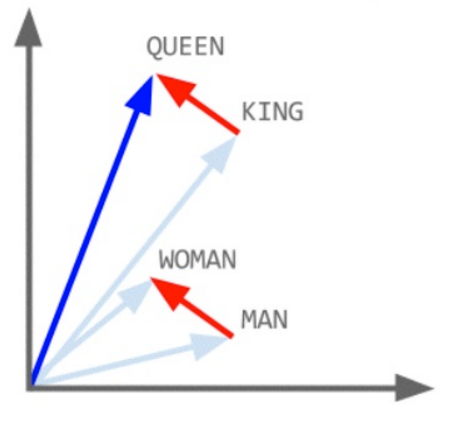
\includegraphics[width = \textwidth]{./Imgs/w2v-example.png}
		\end{column}
	\end{columns}
\end{frame}

\begin{frame}{Word2Vec - RadioCor e Sole 24 Ore - Dettaglio 1}
	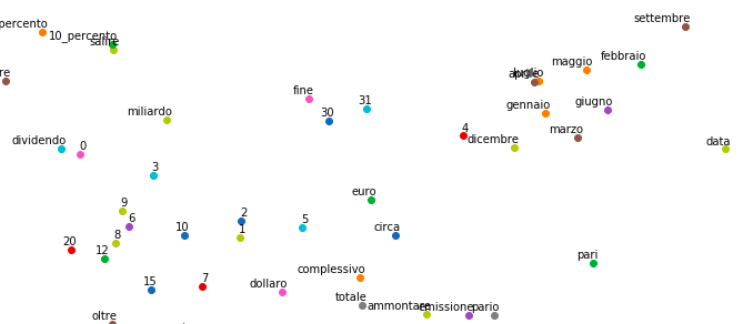
\includegraphics[width = 0.8\textwidth]{./Imgs/plot-numeri.png}
\end{frame}

\begin{frame}{Word2Vec - RadioCor e Sole 24 Ore - Dettaglio 2}
	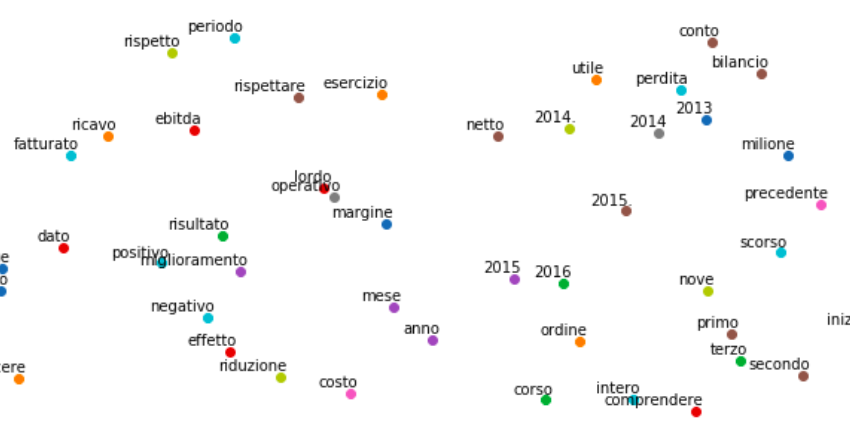
\includegraphics[width= 0.8\textwidth]{./Imgs/plot-anni.png}
\end{frame}

\section{Doc2Vec}

\begin{frame}{Doc2Vec - Task}
	\textbf{Doc2Vec} \`{e} la naturale estensione di \textbf{Word2Vec} che, dato un corpus di \text{documenti}, permette di calcolarne la similarit\`{a}.\\
	\`{E} una \textbf{unsupervised task} che si basa su una \textbf{\alert{two-layers neural network}} che viene trainata su un \textbf{corpora di documenti}. 
	\begin{itemize}
		\item \textbf{Input: }\textbf{corpora} di testi di lunghezza arbitraria
		\item \textbf{Output: }document \textbf{vector-space}
	\end{itemize}	
	Dopo la fase di training ogni documento viene mappato in un vettore colonna della matrice \textbf{D} mentre ogni parola del vocabolario del corpora viene mappata in un vettore colonna della matrice \textbf{W}.	
\end{frame}

\begin{frame}{Doc2Vec - Idea}
	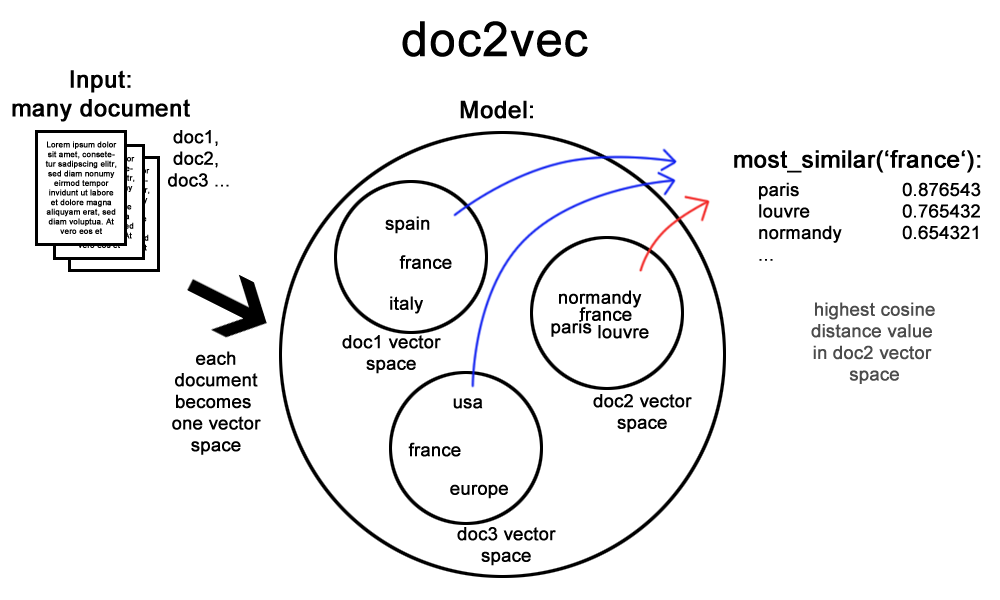
\includegraphics[width=\textwidth]{./Imgs/doc2vec-working.png}
\end{frame}

\begin{frame}{Doc2Vec - CBOW Model}
	L'ispirazione dalla quale nasce \textbf{Doc2Vec} \`{e} \textbf{Word2Vec CBOW}. \\
	Una \textbf{context window} viene fatta scorrere in ogni paragrafo e da essa vengono campionate le parole del contesto $w_{1}, w_{2}, ...,w_{c}$.\\
	Tuttavia, diversamente dal \textbf{CBOW}, la predizione della \textbf{next word} $w_{c+1}$ viene fatta considerando \textbf{le parola precedenti + un vettore caratteristico del paragrafo}.\\
	La struttura \`{e} la seguente:
	\begin{itemize}
		\item \textbf{Input} $w_{1}, w_{2}, ...,w_{c}$ parole nel paragrafo $k$ e il \textbf{Paragraph vector} $p_k $ rappresentante lo specifico paragrafo $k$.
		\item \textbf{Target} \`{e} la prossima parola $w_{c+1}$
	\end{itemize}
\end{frame}

\begin{frame}{Doc2Vec - CBOW Model}
	Le parole nel contesto e il \textbf{Paragraph Vector} vengono concatenate o averaged per predire la prossima parola in un contesto.\\
	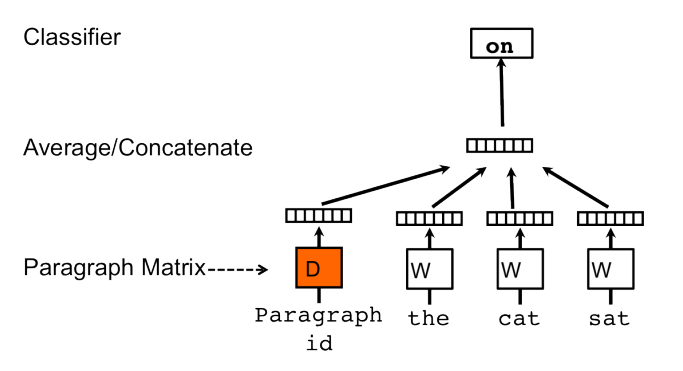
\includegraphics[width= 1.01\linewidth]{./Imgs/d2v-cbow.png}
\end{frame}

\begin{frame}{Doc2Vec - Paragraph token}
	Il \textbf{Paragraph token} pu\`{o} essere visto come una altra parola che agisce da memoria durante la predizione, in modo tale che tenga conto del \textbf{topic} del paragrafo nel quale viene fatta.\\
	Questo modello viene chiamato per questo motivo \textbf{Distributed Memory Model of Paragraph Vectors (PV- DM)}.
\end{frame}

\begin{frame}{Doc2Vec - Skip Grammar}
	\begin{columns}
		\begin{column}{0.5\textwidth}
		Per quanto riguarda l'architettura del \textbf{Skip Gram}, presente gi\`{a} in \textbf{Word2Vec}. \\
		La struttura \`{e} la seguente:
		\begin{itemize}
			\item L'\textbf{input} prevede il \textbf{Paragraph id} che rappresenta lo specifico paragrafo.
			\item L'\textbf{output} sono $w_{1},w_{2},...w_{m}$, parole del paragrafo, dove $\mathrm{M} = window size$
		\end{itemize}
		\end{column}
		\begin{column}{0.5\textwidth}
			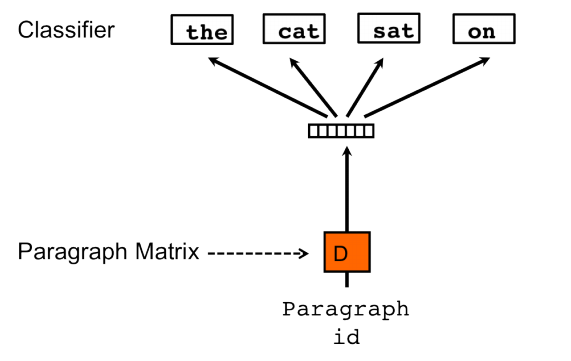
\includegraphics[width=\linewidth]{./Imgs/doc2vec-skipgram.png}
		\end{column}
	\end{columns}
\end{frame}

\begin{frame}{Paragraph Vector}
	Quindi il vettore di ogni parola \textbf{\`{e} condiviso} tra ogni paragrafo.\\
	Mentre il \textbf{Paragraph id}, cio\'{e} la colonna corrispondente al Paragraph nella \textbf{\alert{Paragraph Matrix}}, \textbf{identifica univocamente} ognuno dei paragraph. \\
	Il \textbf{Paragraph id} costituisce una sorta di \textbf{memoria} del topic del paragraph. \\
	Come accade in Word2Vec, tutti i vettori di input sono \textbf{averaged} o \textbf{concatenated}.
\end{frame}

\begin{frame}{Doc2Vec - Risultati}
	Confronto delle performances del Paragraph Vector sull'IMDB dataset.
	Preso da \href{https://cs.stanford.edu/~quocle/paragraph_vector.pdf}{Distributed Representations of Sentences and Documents}
	\centering
	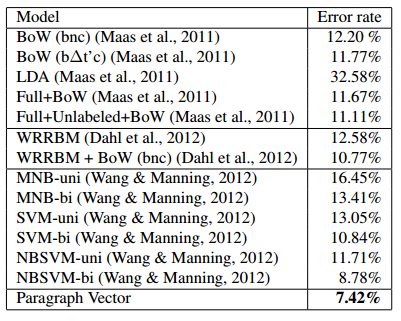
\includegraphics[width = 0.5\linewidth]{./Imgs/d2v-results.png}
\end{frame}

\begin{frame}{References}
	\begin{enumerate}
		\item \href{https://arxiv.org/pdf/1301.3781.pdf}{\textbf{Efficient Estimation of Word Representations in
			Vector Space:} presentazione Skip Gram e CBOW models}
		\item \href{https://papers.nips.cc/paper/5021-distributed-representations-of-words-and-phrases-and-their-compositionality.pdf}{\textbf{Distributed Representations of Words and Phrases
				and their Compositionality:} Word2Vec}
		\item \href{https://cs.stanford.edu/~quocle/paragraph_vector.pdf}{\textbf{Paragraph Vectors}}
		\item \href{https://arxiv.org/pdf/1507.07998.pdf}{\textbf{Document Embedding with Paragraph Vectors:} Doc2Vec}
	\end{enumerate}
\end{frame}

\end{document}
